Tugas akhir ini memanfaatkan model simulasi perangkat keras dan perangkat lunak yang dikonfigurasi dalam lingkungan Mujoco. Perangkat keras yang disebutkan merupakan model digital yang digunakan dalam simulasi, bukan perangkat fisik yang dioperasikan secara langsung.

\subsection{Model robot hexapod sebagai platform navigasi}

Model robot hexapod pada lingkungan simulasi Mujoco digunakan sebagai platform utama. Model ini merepresentasikan robot hexapod berkaki enam yang masing-masing dapat dikendalikan secara individual, sehingga mampu menyesuaikan postur dan posisi saat berpindah antar region atau lapisan \emph{costmap}. Model robot ini dipilih karena sesuai dengan karakteristik gerak yang dibutuhkan untuk navigasi di medan tidak rata.

\begin{figure}[H]
\centering
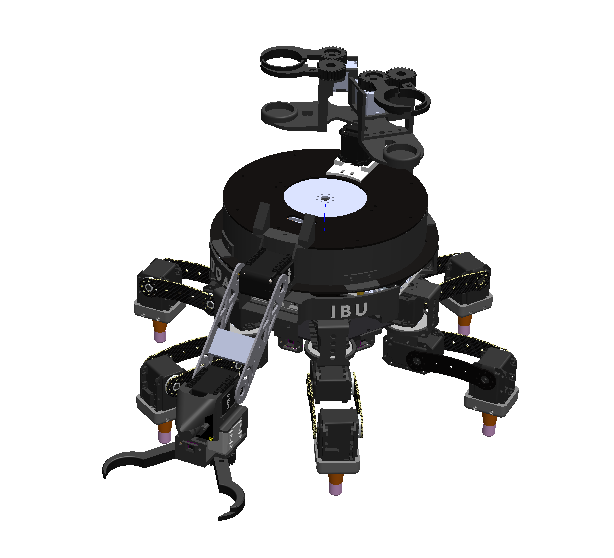
\includegraphics[scale=0.6]{gambar/platform_robot.png}
\caption{Model platform navigasi yang digunakan dalam simulasi}
\label{fig:platform_robot}
\end{figure}

\subsection{Sensor LiDAR 2D pada lingkungan simulasi}

Sensor LiDAR 2D pada lingkungan simulasi dikonfigurasi untuk mendeteksi rintangan di sekitar robot secara \emph{real-time}. Sensor bekerja dengan memancarkan sinar laser virtual dan mengukur jarak ke objek di sekitarnya. Data hasil pembacaan digunakan sebagai masukan untuk membentuk \emph{costmap} dan deteksi rintangan pada sistem navigasi.

Parameter sensor yang digunakan dalam simulasi disetarakan dengan spesifikasi YDLiDAR T-mini-plus, yaitu frekuensi \emph{scan} 12 Hz, \emph{scan angle} $360^\circ$, resolusi sudut $0.54^\circ$, dan jarak maksimum 12 m.

\begin{figure}[H]
\centering
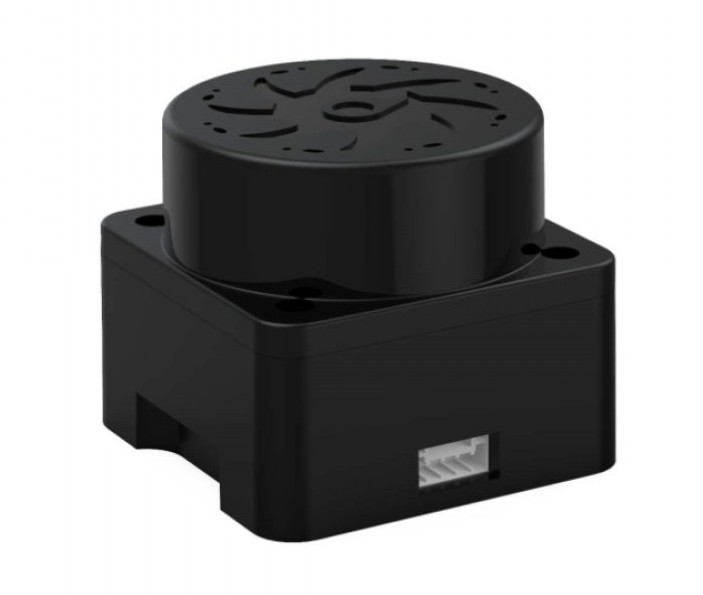
\includegraphics[scale=0.4]{gambar/ydlidar-t-mini-plus.jpg}
\caption{Sensor YDLiDAR T-mini-plus sebagai referensi parameter LiDAR 2D pada simulasi \parencite{ShenzhenEAITechnology2024ydlidar}}
\label{fig:ydlidar}
\end{figure}

\subsection{Perangkat lunak pendukung}

Penelitian ini menggunakan beberapa perangkat lunak pendukung yang saling
terintegrasi untuk membangun sistem navigasi robot otonom, yaitu:

\begin{enumerate}
  \item \textbf{ Robot Operating System (ROS) Noetic},
  merupakan \emph{middleware} yang menyediakan kerangka kerja
  (\emph{framework}) komunikasi antarproses dalam sistem robot.
  Pada penelitian ini, ROS Noetic digunakan sebagai basis integrasi
  seluruh komponen sistem, mulai dari pembacaan sensor LiDAR,
  lokalisasi ICP, pengelolaan \emph{costmap}, perencanaan jalur,
  hingga kendali robot.

  \item \textbf{Simulator MuJoCo (Multi-Joint dynamics with Contact)}, adalah \emph{physics simulator} yang digunakan untuk
  menjalankan simulasi lingkungan dan dinamika robot. Seluruh
  pengujian dalam penelitian ini dilakukan di dalam MuJoCo, termasuk
  pergerakan robot hexapod, pembacaan sensor LiDAR, dan interaksi
  robot dengan lingkungan simulasi.

  \item \textbf{RViz}, merupakan perangkat lunak visualisasi
  dari ROS yang digunakan untuk menampilkan data sensor, posisi
  robot, \emph{costmap}, serta jalur navigasi secara grafis.
  Dengan RViz, pengguna dapat memonitor pergerakan robot dan
  memverifikasi apakah sistem navigasi dan lokalisasi berjalan
  dengan benar dalam lingkungan simulasi.

  \item \textbf{ROS Navigation Stack}, adalah
  \emph{library} yang menyediakan kerangka kerja untuk navigasi
  robot bergerak. Komponen utama yang digunakan dalam penelitian ini
  meliputi move base sebagai \emph{action server} yang
  mengelola pipeline navigasi, serta costmap2d sebagai
  implementasi \emph{layered costmap} yang menjadi dasar representasi
  lingkungan.
\end{enumerate}

% \subsection{Lingkungan simulasi}

% Lingkungan simulasi dalam penelitian ini diadaptasi dari arena Kontes Robot SAR Indonesia (KRSRI) 2024. Arena didesain untuk merepresentasikan kondisi area pasca bencana dalam skala laboratorium, mencakup beberapa elevasi seperti tanjakan, permukaan tidak rata, dan rintangan yang meniru situasi nyata secara sederhana. Arena tersebut dimodelkan ulang di dalam simulator Mujoco untuk keperluan pengujian sistem navigasi.

% \begin{figure}[H]
% \centering
% 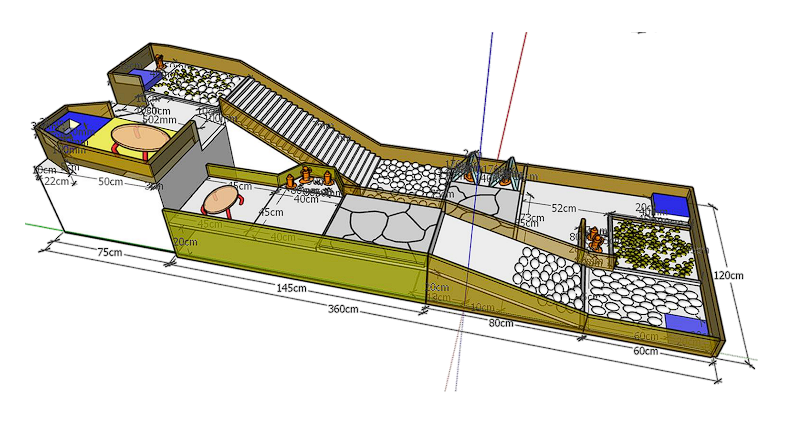
\includegraphics[scale=0.65]{gambar/arena_with_dimension.png}
% \caption{Sketsa arena laboratorium KRSRI 2024 yang digunakan sebagai acuan lingkungan simulasi \parencite[]{KRI2024Pedoman}}
% \label{fig:arena_with_dimension}
% \end{figure}